\documentclass[tikz, border=1pt]{standalone}
\pdfoutput=1 % if your are submitting a pdflatex (i.e. if you have
             % images in pdf, png or jpg format)

\usepackage{graphicx}

% Use the tikz package
\usepackage{tikz}
\usetikzlibrary{decorations}


\begin{document}

	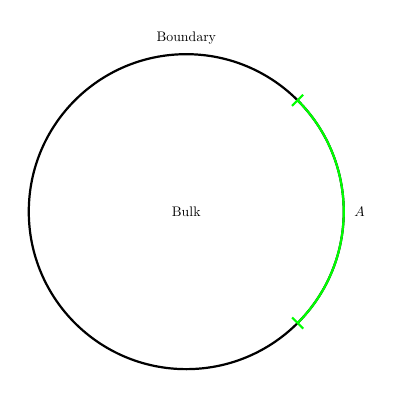
\begin{tikzpicture}
        
        %The boundary circle
        \draw [thick] (0,0) circle (2);
        
        % The RT Surface
		%\draw [thick,blue] (2.82843,0) ++(135:2) arc (135:225:2);
		
		% The region
		\draw [thick,green] (0,0) ++(45:2) arc (45:-45:2);
		\draw [thick,green] (0,0) ++(45:1.9)--(45:2.1);
		\draw [thick,green] (0,0) ++(-45:1.9)--(-45:2.1);
        
        %labels
        \draw (2.2, 0) node[scale = 0.5]{$A$};
        \draw (0, 0) node[scale = 0.5]{Bulk};
        \draw (0, 2.2) node[scale = 0.5]{Boundary};
        %\draw (1, 0) node[scale = 0.5]{RT};
		
	\end{tikzpicture}

\end{document}
